\section{Введение}

\begin{frame}{Сравнивать картинки сложно!}

\begin{itemize}
    \item Компьютер не понимает смысла картинок.
    \item Две <<похожие>> картинки могут иметь сильные отличия.
\end{itemize}

\centering
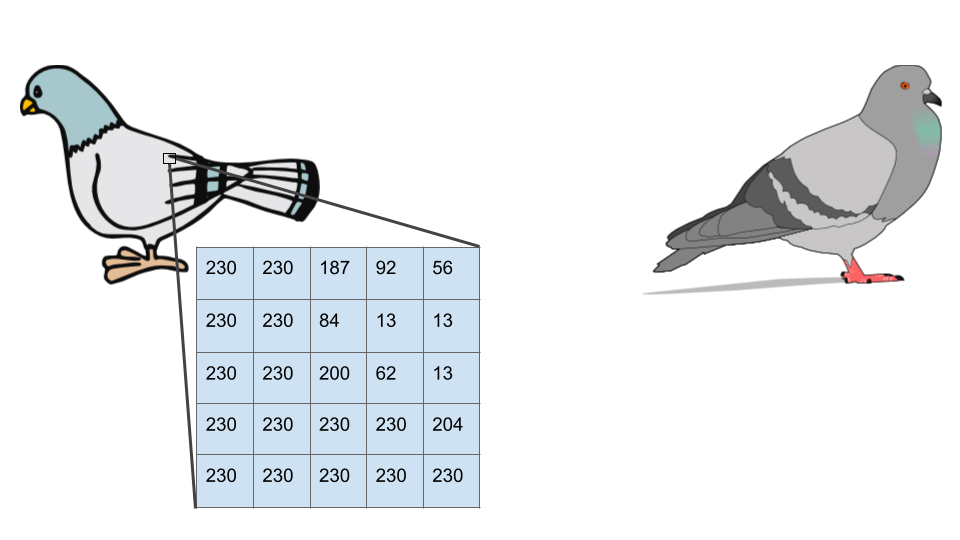
\includegraphics[width=0.8\textwidth]{images/pigeon start.png}
\end{frame}

\begin{frame}{Сопоставление шаблона}
Можно искать определённый шаблон на картинке скользящим окном:
\begin{itemize}
    \item Через корреляцию шаблона и текущего положения окна.
    \item Или через квадрат разницы.
\end{itemize}

\centering
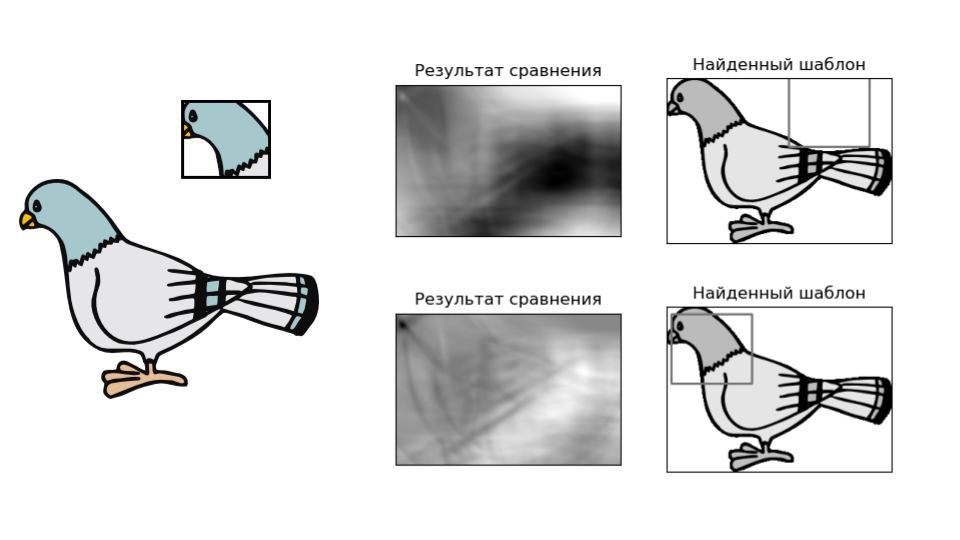
\includegraphics[width=0.8\textwidth]{images/pigeon template matching.png}

\alternativefootnote{\url{https://docs.opencv.org/master/d4/dc6/tutorial_py_template_matching.html}}
\end{frame}

\begin{frame}{Сопоставление шаблона}

\begin{itemize}
    \item Подправим способ сравнения, учтя общую освещённость.
    \item Для корреляции это помогло найти правильное местоположение.
\end{itemize}

\centering
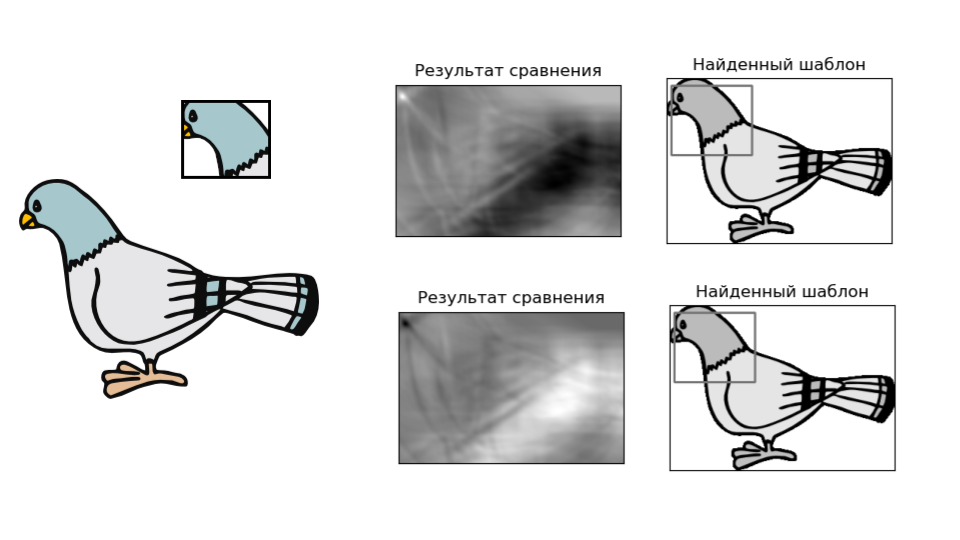
\includegraphics[width=0.8\textwidth]{images/pigeon template matching2.png}

\alternativefootnote{\url{https://docs.opencv.org/master/d4/dc6/tutorial_py_template_matching.html}}
\end{frame}
